% !TEX program = xelatex
% basic document config
\documentclass[a4paper,10pt,xetex]{article}
\usepackage[a4paper,top=45mm,right=20mm,bottom=30mm,left=25mm,head=35mm,foot=20mm]{geometry}

% language
\usepackage[german]{babel}

% variable definitions
\providecommand{\documenttitle}{Design}
\providecommand{\documentauthors}{Andreas Saurer \\ Benjamin Schneidinger \\ Josef Erben \\ Raffaele Bof \\ Nicolas Loth}
\providecommand{\documentdate}{25.04.2017}

% special commands
\newcommand*{\fullref}[1]{\hyperref[{#1}]{\nameref*{#1} (\ref*{#1})}}
\newcommand{\specialcell}[2][c]{%
  \begin{tabular}[#1]{@{}l@{}}#2\end{tabular}}

% font
% \usepackage{titling}
\usepackage[sfdefault]{roboto}
\usepackage[parfill]{parskip}

% table
\usepackage{array}
\usepackage{multicol}
\usepackage{longtable,tabu,booktabs}

% links
\usepackage{hyperref}
\hypersetup{
            pdftitle={\documenttitle},
            pdfauthor={\documentauthors},
            colorlinks=true,
            linkcolor=[RGB]{74,144,226},
            citecolor=[RGB]{74,144,226},
            urlcolor=[RGB]{74,144,226},
            breaklinks=true}
\urlstyle{same}  % don't use monospace font for urls

% images
\usepackage{float,graphicx,grffile}
\graphicspath{ {images/} }

\makeatletter
\def\maxwidth{\ifdim\Gin@nat@width>\linewidth\linewidth\else\Gin@nat@width\fi}
\def\maxheight{\ifdim\Gin@nat@height>\textheight\textheight\else\Gin@nat@height\fi}
\makeatother
\setkeys{Gin}{width=\maxwidth,height=\maxheight,keepaspectratio}

\makeatletter
\def\fps@figure{H}
\makeatother

% header and footer
\usepackage{lastpage}
\usepackage{fancyhdr}
\pagestyle{fancy}
\fancyhf{}
\fancyhead[L]{
\includegraphics[height=2cm]{travel-buddy_white}}
\fancyfoot[L]{\fontsize{8}{10}\selectfont\ \documenttitle}
\fancyfoot[R]{\fontsize{8}{10}\selectfont\ Seite\ \thepage\ von\ \pageref*{LastPage}}

\renewcommand{\headrulewidth}{0pt}
\renewcommand{\footrulewidth}{0pt}

% style titles
\usepackage{titlesec}
\titlespacing*{\section}{0pt}{1em}{0pt}
\titlespacing*{\subsection}{0pt}{1em}{0pt}
\titlespacing*{\subsubsection}{0pt}{1em}{0pt}

% configure title page
\title{
  
\includegraphics[width=7cm]{travel-buddy_white}\\[\bigskipamount]
  Anforderungsanalyse\\[\bigskipamount]
}

\author{\documentauthors}
\date{\parbox{\linewidth}{\centering%
  IT15TA ZH \hspace*{3cm} Gruppe 3\endgraf\bigskip
  \documentdate\endgraf
}}


\begin{document}

% title page
\maketitle\newpage

% table of contents
{
\hypersetup{linkcolor=black}
\setcounter{tocdepth}{3}
\tableofcontents
}

\newpage

% version log
\section{Versionenlog}\label{versionenlog}

\tabulinesep=1.2mm

\begin{longtabu} to \textwidth { | l | l | X[l] | l | }
  \hline
  \textbf{Datum} & \textbf{Version} & \textbf{Änderung} & \textbf{Author} \\
  \hline
  \endhead

  0.0.5 & 23.04.2017 & Klassendiagramm Frontend erstellt und hinzugefügt & Josef \\
  \hline

  0.0.4 & 23.04.2017 & Interaktionsdiagramme zusammengetragen und hinzugefügt & Andi \\
  \hline

  0.0.3 & 23.04.2017 & Implikationen der Frontend Architektur, Nachtrag Glossar & Josef \\
  \hline

  0.0.2 & 22.04.2017 & Initiale Version der Frontend Architektur & Josef \\
  \hline

  0.0.1 & 21.04.2017 & GUI-Design Text hinzugefügt & Andi\\
  \hline

  0.0.0 & 21.04.2017 & Dokument erstellt & Andi\\
  \hline
\end{longtabu}
\newpage

% start content
\section{Projektmanagement}\label{projektmanagement}
\section{Architektur}\label{architektur}
\subsection{Android App Architektur}\label{androidapparchitektur}

Die Architekur der App implementiert eine einfache Version von \textbf{The Clean Architecture} [2].
Im nachfolgenden Abschnitt werden einige wichtige Punkte von \textbf{The Clean Architecture}
erläutert, um die Implementation in TravelBuddy aufzuzeigen. Eine umfassende
Einleitung findet man bei Robert Martin (Uncle Bob) [3].
\begin{figure}
  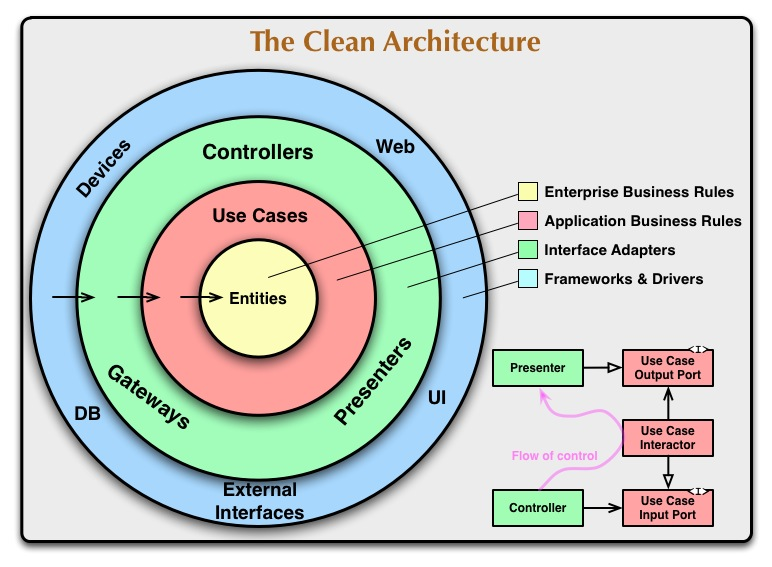
\includegraphics{cleanarchitecture}
  \caption{Schema von The Clean Architecture}
\end{figure}

\subsubsection{Abhängigkeiten - Dependency Rule}\label{dependencyrule}
Diese einfache Regel stellt lose Kopplung und gute Testbarkeit sicher.
Die \textbf{Dependency Rule} besagt, dass die Source Code Abhängigkeit nach innen zeigt.
Das heisst, dass eine bestimmte Schicht niemals die äussere Schicht kennt.
Man hat beispielsweise einen HTTP Client (Web) in der äussersten Schicht und
einen Parser (Gateway) in der direkt darunterliegenden Schicht. Nach der
\textbf{Dependency Rule} darf es keine Referenzen im Parser zum HTTP-Client geben.

\subsubsection{Bedeutung der Schichten}\label{layers}
\begin{longtabu} to \textwidth { | l | X[l] |  }
\hline
\textbf{Bezeichnung der Schicht} & \textbf{Bedeutung und Beispiele}\\\hline
\endhead
\textbf{Frameworks and Drivers} & Die äusserste Schicht \textbf{Frameworks and Drivers}
ist für die Kommunikation mit der äusseren Welt zuständig. Dazu zählen zum
Beispiel Kommunikation mit dem User per UI, Persistierung von Daten in Datenbanken
oder Kommunikation mit externen Services per HTTP. Die äusserste Schicht beinhaltet
aber auch Frameworks.\\\hline
\textbf{Interface Adapters} & Die nachfolgende Schicht heisst \textbf{Interface Adapters}.
Diese Schicht hat zur Aufgabe, die Daten in eine für die Use Cases und Entities
möglichst angenehme Form zu bringen.\\\hline
\textbf{Use Case} & Der zweitinnerste Schicht nennt man \textbf{Use Case} Layer.
Hier werden die applikationsspezifischen Businessregeln, also die Use Cases abgebildet.
Die eigentliche Businesslogik existiert also in dieser Schicht. Zu beachten ist aber,
dass es hier nur um Verhalten und nicht um Daten geht.\\\hline
\textbf{Entities} & Die eigentlichen Businessobjekte gehören in die innerste
Schicht genannt \textbf{Entities}. Diese Schicht hat keine Abhängigkeiten zu
anderen Schichten und beinhaltet die generellen Regeln der Domäne. Bei Änderungen
in äusseren Schichten sind mit hoher Wahrscheinlichkeit keine Änderungen in dieser
Schicht notwendig. Zur Abgrenzung zur oberen Schicht \textbf{Use Case}: Die Schicht \textbf{Entities}
muss nicht angepasst werden, falls sich Use Cases ändern. Dies is der Fall, da
sich die allgemeinen Domänenregeln in der Regel nicht ändern.\\\hline
\end{longtabu}

\subsubsection{The Clean Architecture bei TravelBuddy}
Die TravelBuddy App ist ein Spezialfall einer Android App. Da das Team das grösste
Risiko bei der Android-Entwicklung sah, wurde entschlossen in der App selber so
wenig Businesslogik wie möglich auszuführen.
Dies hat natürlich einen Einfluss auf die Architektur, wie im folgenden Abschnitt aufgezeigt wird.


\subsubsection{Schichten}\label{layerstravelbuddy}
\begin{longtabu} to \textwidth { | l | X[l] |  }
\hline
\textbf{Schicht} &  \textbf{Zuständigkeiten und Beispiele} \\\hline
\endhead
\textbf{Frameworks and Drivers} & Kümmert sich um Lifecycle der App, die Berechtigungen
und um die Einbettung ins Android Betriebssystem, setzt HTTP Requests ab und reicht
HTTP Responses weiter, aktualisiert Standortdaten, bekommt Bilder von der
Smartphone-Kamera, erhält Karte von der Google Maps App\\\hline
\textbf{Interface Adapters} & Parst Antwort des Servers in String-Form und wandelt
diese Datenobjekte um, transformiert Kartendaten und Standortdaten in für die App
einfach zu handhabbare Form\\\hline
\textbf{Use Case} & Hier kommt der einfache Fall der Android App zugute: Die App
enthält sehr wenig Businesslogik. Die Use Cases sind im Backend implementiert.\\\hline
\textbf{Entities} & Enthählt die Datenobjekte, welche die Domänenregeln abbilden:
Eine Tour besteht aus einer Liste von Routen, jede Route hat ein POI zum Ziel\\\hline
\end{longtabu}

\subsubsection{Implikationen}\label{implications}
Die Anwendung der \textbf{Clean Architecture} bringt natürlich sowohl Vor- als
auch Nachteile. Die nachfolgende Liste zeigt Implikationen und Auswirkungen der
gewählten Architektur auf das Design und die Umsetzung der App.
\begin{enumerate}
  \item \textbf{Klare Abhängigkeiten:} Durch die klar definierten Abhängikeiten
    lassen sich Kosten und Aufwände von Änderungen/Erweiterungen besser abschätzen:
    Wollen wir beispielsweise die Technologie zur Kommunikation mit dem
    Backend von REST/HTTP auf WebSockets/PubSub ändern, wissen wir, dass sich
    die inneren beiden Schichten nicht ändern. Wir müssen lediglich die äussere
    Schicht anpassen, damit sie WebSockets handhabt. Der Parser, in der direkt
    darunterliegenden Schicht, erhält idealerweise den gleichen Response Body
    und muss nicht angepasst werden.
  \item \textbf{Gute Testbarkeit:} Die Businesslogik ist vollkommen unabhängig
    von verwendeteten Frameworks und der UI. Diese kann ohne eine laufende
    Android Instanz getestet werden. Das führt zu kürzeren Feedback Loops
    bei der Ausführung von Unit Tests und dadurch zur effizienteren Entwicklung.
    (Ein komplettes Re-deployment entfällt)
    Da in den beiden inneren Schichten keine Abhängigkeit zu externen Systemen
    besteht, lassen sich diese ohne grossen Aufwand (z.B. Testing-Setup) testen.
  \item \textbf{Keine Abhängikeit zum Betriebssytem:} Aus Punkt 1 und 2
    leitet sich dieser Punkt ab: Alle Abhängigkeiten befinden sich um
    äussersten Layer. Falls die App auch auf anderen Systemen lauffähig sein soll,
    dann muss im Idealfall nur eine Schicht angepasst werden. Durch Projekte
    wie RoboVM und Intel Multi OS Engine können wir den bestehenden Java Code
    sogar auf iOS Geräten laufen lassen. Unsere App ist damit sogar nur lose
    zum Betriebssystem gekoppelt.
  \item \textbf{Overhead:} Da die App in der ersten Version praktisch keine
    Businesslogik enthalten wird, entfällt die \textbf{Use Case} Schicht.
    Dadurch bleiben eigentlich die anderen drei Layer, die mit der ersten
    Version ebenfalls noch Überschaubar ausfallen. Man könnte argumentieren,
    dass diese Architektur etwas zu hoch gegriffen ist für die Anforderungen
    des Prototypen. Im Gegensatz zu Design lässt sich Architektur nicht oder
    sehr schwer iterativ entwickeln. Wir denken, dass der Aufwand für Änderungen
    der Architektur im späteren Verlauf (etwa durch neue Anforderungen) den
    initialen Mehraufwand rechtfertigt.
\end{enumerate}

Durch die gewählte Architektur erreichen wir gute Testbarkeit mit klaren
Abhängigkeiten. Der Mehraufwand wird dadurch gerechtfertigt, dass Änderungen
von Technologien nur kleine, kalkulierbare Anpassungen zur Folge haben.

\section{Design-Klassendiagramm}\label{design-klassendiagram}
\subsection{Design-Klassendiagramm Frontend}\label{design-klassendiagram-frontend}
\begin{figure}
  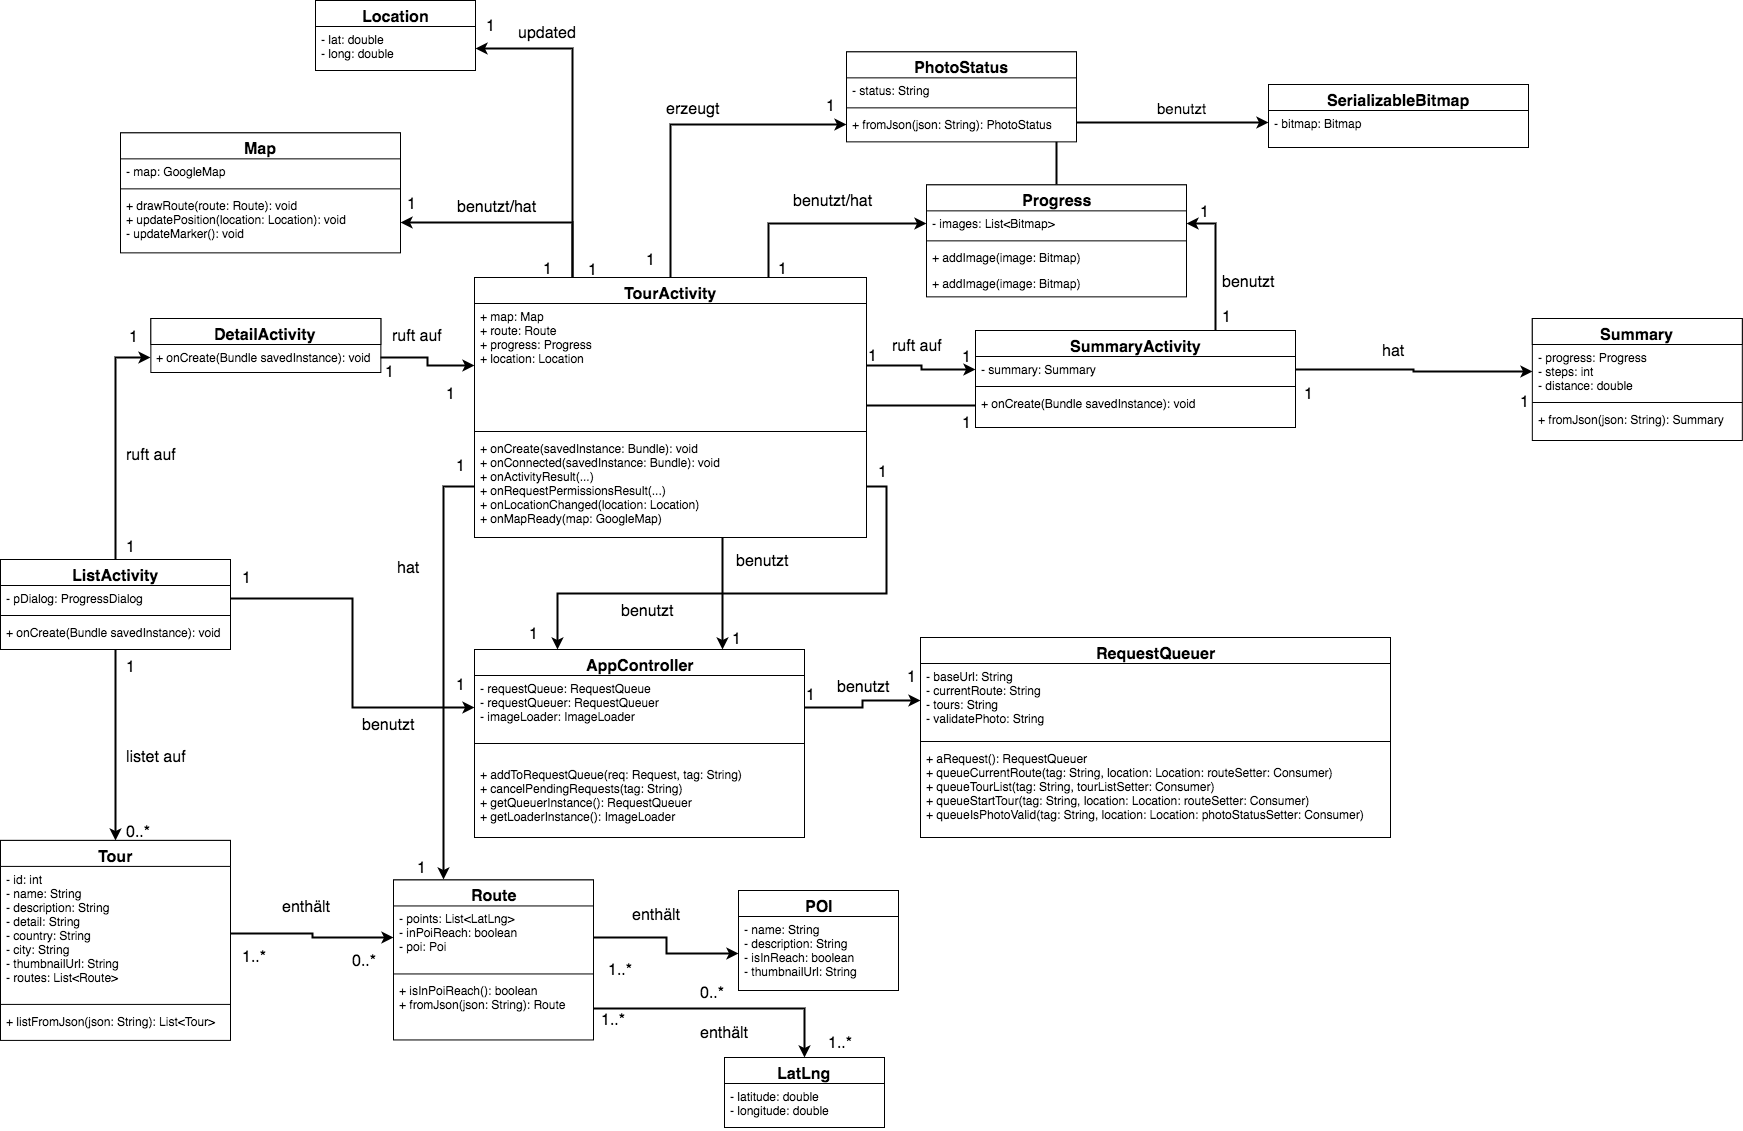
\includegraphics{classdiagram_frontend}
  \caption{Klassendiagramm der App}
\end{figure}

\section{Klassenverantwortlichkeiten}\label{klassenverantwortlichkeiten}
\subsection{Klassenverantwortlichkeiten - App}\label{klassenverantwortlichkeiten-frontend}
In der folgenden Tabelle werden die Klassen mit ihren Hauptverantworlichkeiten
gelistet.

\begin{longtabu} to \textwidth { | l | X[l] |  }
\hline
\textbf{Klasse} & \textbf{Verwantwortlichkeit}\\\hline
\endhead
\textbf{AppController} & Der AppController liefert Instanzen von Singletons.\\\hline
\textbf{RequestQueuer} & Der RequestQueuer wird benutzt, um per HTTP mit dem 
Server zu kommunizieren.\\\hline
\textbf{ListActivity} & Die ListActivity zeigt eine Liste von Touren an und 
reagiert auf Klick-Events.\\\hline
\textbf{DetailActivity} & Die DetailActivity zeigt eine detaillierte Beschreibung 
und ein Thumbnail einer Tour.\\\hline
\textbf{TourActivity} & Die TourActivity speichert die aktuelle Route, aktualisiert
die Position des Nutzers, aktualisiert die Karte und löst HTTP Requests aus.\\\hline
\textbf{SummeryActivity} & Die SummaryActivity erstellt eine \textbf{Summary} 
und zeigt diese an.\\\hline
\textbf{Tour} & Die Tour kennt all ihre Routen und dient als Datenklasse. \\\hline
\textbf{Route} & Die Route kennt all ihre Koordinaten und dient als 
Datenklasse. \\\hline
\textbf{POI} & Die POI ist eine reine Datenklasse und bildet ein POI ab.\\\hline
\textbf{LatLng} & LatLng ist ein Datentyp, welche eine Position auf dem
Erdball abbildet.\\\hline
\textbf{Map} & Die Map dient als Behählter der Google Map und wird benutzt, um
die Karte zu aktualisieren.\\\hline
\textbf{Location} & Location ist eine Repräsentation einser Ortes und kommt aus 
Android SDK.\\\hline
\textbf{PhotoStatus} & PhotoStatus ist ein Datenobjekt und repräsentiert das 
Ergebnis einer Validation eines Fotos durch das Backend.\\\hline
\textbf{Progress} & Progress dient als Behälter der während einer Tour geschossenen
Fotos.\\\hline
\textbf{Summary} & Summary wird am Ende einer Tour aus Progress generiert und
bietet dem Nutzer eine Zusammenfassung der Tour.\\\hline
\end{longtabu}

\subsubsection{Klassenverantwortlichkeiten - Knowing and Doing}\label{knowinganddoing-frontend}
Im Folgenden betrachten wie die Knowing- und Doing-Verantwortlichkeiten der Klassen. 
\begin{longtabu} to \textwidth { | l | l | X[l] |  }
\hline
\textbf{Klasse} & \textbf{Knowing} & \textbf{Doing} \\\hline
\endhead
\textbf{AppController} & RequestQueuer & Stellt anderen Objekten den RequestQueuer 
als Singleton zur Verfügung\\\hline
\textbf{RequestQueuer} & keine Abhängigkeiten & Wird in den Activities für asynchrone
HTTP Kommunikation benutzt. Der RequestQueuer baut auch die URLs zusammen und bietet
eine API an, um mit Lambdas Callbacks zu setzen. Dieser ruft die mitgereichten 
Consumer mit dem Server Response auf, ohne den Aufrufer zu kennen. Dadurch erreichen
wir lose Kopplung und hohe Wiederverwandbarkeit. \\\hline
\textbf{ListActivity} & AppController, Tour & Die ListActivity gibt über den AppController
einen Callback an den RequestQueuer. Dieser Callback füllt eine Liste von Touren,
welche dem User angezeigt wird. Ein Kick auf eine Tour ruft die DetailActivity auf.
\\\hline
\textbf{DetailActivity} & Tour & Die DetailActivity ist eine einfache Ansicht auf 
ein Tour-Objekt und zeigt Details einer Tour an.\\\hline
\textbf{TourActivity} & Map, Route, Progress, Location, AppController & Die TourActivity bildet
unseren Hauptusecase ab: Navigation per Karte durch eine Tour. Die TourActivity
registriert sich selber als Callback beim Google Maps Service und beim Google
Play Location Service. Weiterhin wird das Backend regelmässig nach der aktuellen
Route gefragt. Falls sich der User in der Nähe eines Pois befindet, wird die 
Kamera App des Smartphones aktiviert.\\\hline
\textbf{SummeryActivity} & Summary, Progress, RequestQueuer & Die SummaryActivity 
bekommt von der TourActivity ein Progress-Objekt. Nach einer Anfrage an das 
Backend wird eine \textbf{Summary} Activity erstellt und angezeigt.\\\hline
\textbf{Tour} & Route & Die Tour kennt nur ihre Routen und dient als Datenklasse. 
Sie kann sich selber aus JSON instanziieren.\\\hline
\textbf{Route} & LatLng & Die Route kennt all ihre Koordinaten und dient als 
Datenklasse. Sie kann sich selber aus JSON instanziieren.\\\hline
\textbf{POI} & keine Abhängigkeiten & Die POI ist eine reine Datenklasse und bildet ein POI ab. Sie 
kann sich selber aus JSON instanziieren.\\\hline
\textbf{LatLng} & keine Abhängigkeiten & LatLng ist ein Datentyp, welche eine Position auf dem
Erdball abbildet.\\\hline
\textbf{Map} & GoogleMap & Die Map dient als Behählter der Google Map und wird benutzt, um
die Karte zu aktualisieren. Sie kann den Positionsmarker und die Route zum nächsten
POI zeichnen.\\\hline
\textbf{Location} & keine Abhängigkeiten & kein Verhalten \\\hline
\textbf{PhotoStatus} & keine Abhängigkeiten & kein Verhalten \\\hline
\textbf{Progress} & keine Abhängigkeiten & kein Verhalten \\\hline
\textbf{Summary} & Progress & Summary kann sich selber aus \textbf{Progress} 
generieren.\\\hline
\end{longtabu}

Obwohl \textbf{Activities} andere \textbf{Activites} starten können, müssen sie
lediglich deren Klasse kennen. Durch das Messaging System von Android müssen die
Activities keine Instanzen von anderen Activities halten oder diese selber 
erzeugen. Im Klassendiagramm (Abbildung 2) sind die Activities zwar miteinander
verbunden, aber durch das Message System (Intents) sind diese lose gekoppelt.

\section{Interaktionsdiagramme}\label{interaktionsdiagramme}
\subsection{Backend}\label{backend}

\subsubsection{Tour starten}
\begin{figure}
  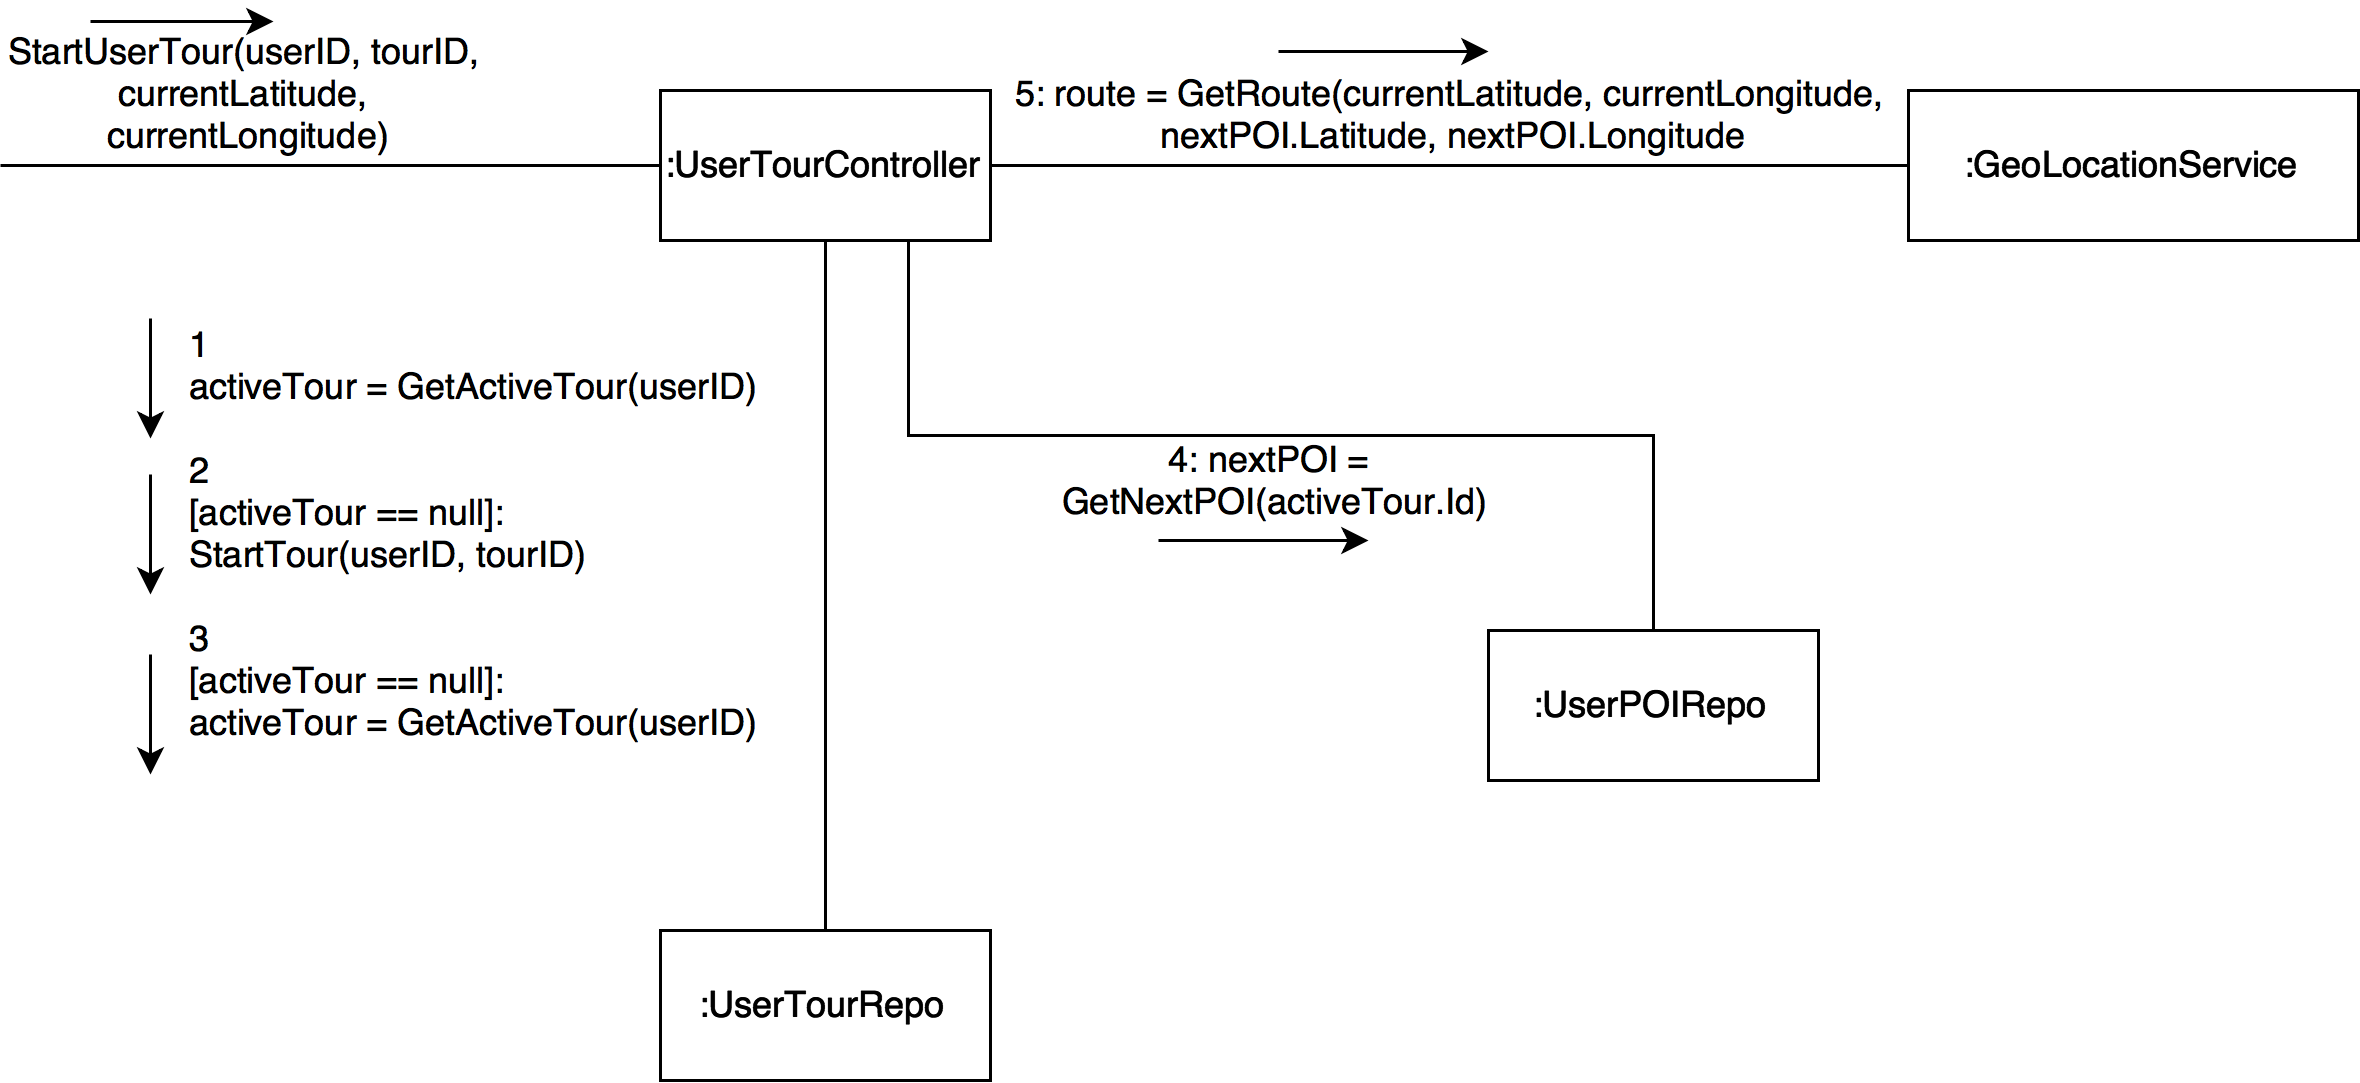
\includegraphics{Kommunikationsdiagramm_StartTour}
  \caption{Kommunikationsdiagramm Tour starten}
\end{figure}

\subsubsection{Route zu PoI}
\begin{figure}
  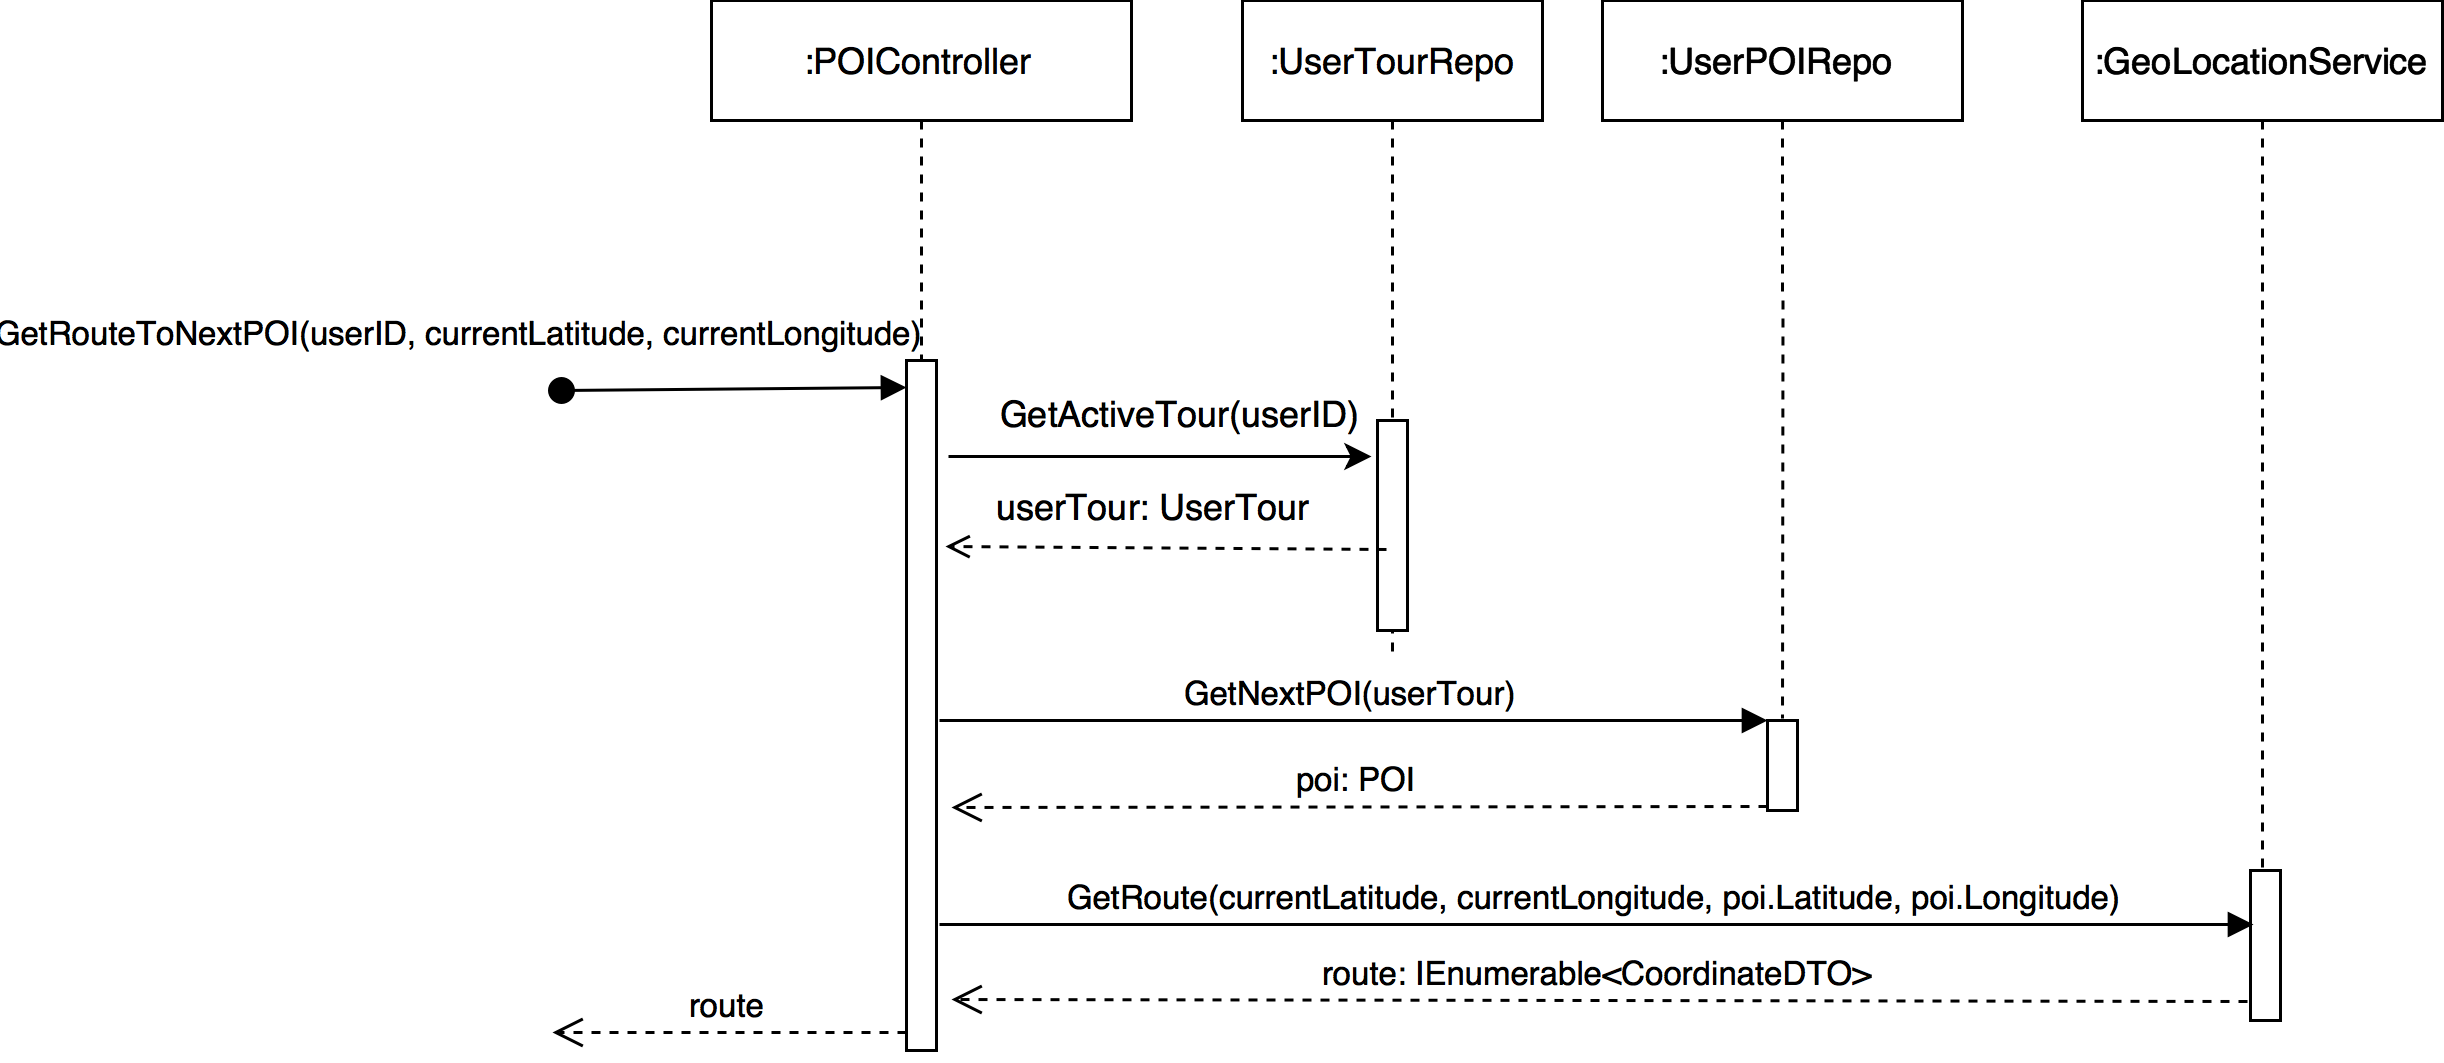
\includegraphics{Sequenzdiagramm_GetRouteToPoi}
  \caption{Sequenzdiagramm Route zu PoI}
\end{figure}

\subsection{Frontend}\label{frontend}
\subsubsection{Tour Liste anzeigen}
\begin{figure}
  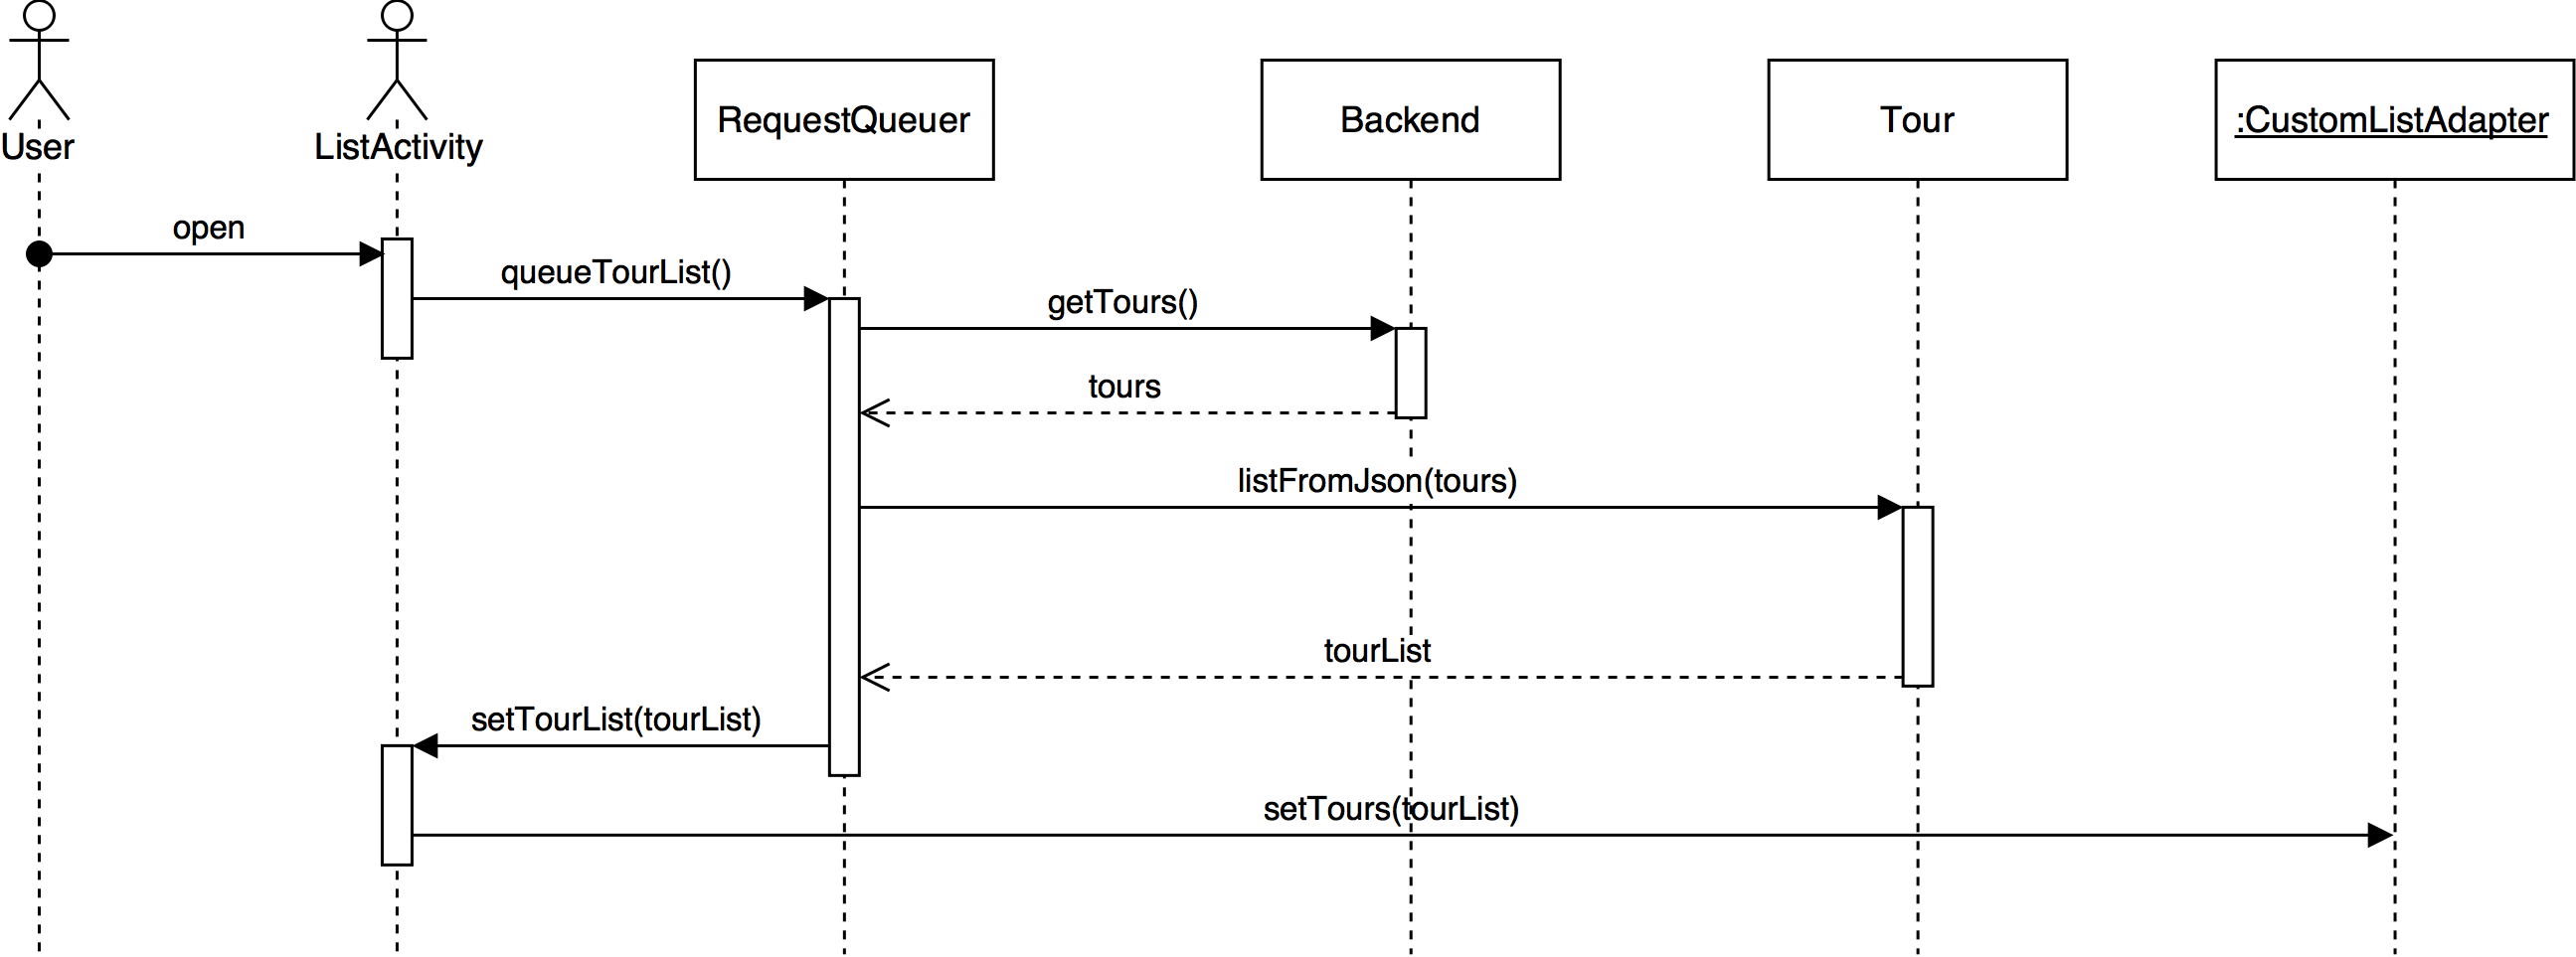
\includegraphics{Sequenzdiagramm_getTours}
  \caption{Sequenzdiagramm Tour Liste anzeigen}
\end{figure}

\section{GUI-Design}\label{gui-design}
Die App startet auf der Anzeige ``ListActivity'' auf welchem alle verfügbaren Touren angezeigt
werden. Mit einem Klick auf eine Tour wird die Anzeige ``DetailActivity'' geöffnet und eine
Übersicht über die gewählte Tour wird sichtbar. Über den Button ``Tour starten'' gelangt
man weiter zur Ansicht ``TourActivity'' worauf jeweils der Weg zum nächsten POI ersichtlich ist.
Abgeschossen wird eine Tour mit der Anzeige ``SummaryActivity''.

\newpage
\section{Glossar}\label{glossar}
\begin{longtabu} to \textwidth { | l | X[l] | }
\hline
\textbf{Begriff} & \textbf{Bemerkung}\\\hline
\endhead

Agency/Agencies & engl. Agenturen\\\hline
Smartphone & Mobilgerät mit erweiterten Funktionen\\\hline
Android & Betriebssystem für Mobilgeräte\\\hline
Mobile Application/Mobile App & Mobile Applikation, Synonym für mobile Applikation auf Smartphone\\\hline
Backend & Serverseitige Anwendung, stellt Rest API zur Verfügung\\\hline
External Services & engl. Externe Dienste, Dienste die nicht vom Programm selber ausgeführt werden wie z.B. Location Services\\\hline
Fallback & Ausweichlösung/Alternativlösung\\\hline
Frontend & Benutzerseitige Anwendung, hier App welche Rest API konsumiert\\\hline
GPS & Global Positioning System, globales Satelliten Navigationsnetz\\\hline
Marker & Symbol, welches einen Punkt auf der Karte markiert\\\hline
Natives Features & Funktionen, die ein Gerät ohne weitere Software besitzt\\\hline
ÖV & abkz. Öffentlicher Verkehr\\\hline
Point of Interest, PoI & engl. Ort von besonderem Interesse, bspw. Wahrzeichen\\\hline
Stakeholders & engl. Interessenten\\\hline
Tech Stack & Eingesetzte Technologien\\\hline
Mockdaten & Daten mit gleicher Struktur wie echte Daten, dient der lokalen Entwicklung, Testdaten \\\hline
Trip & engl. Reise, enthält mehrere Touren\\\hline
Tourist & Der eigentliche Benutzer der App\\\hline
POJO & Plain old Java object (Datenobjekt)\\\hline
PubSub & Publisher subscriber Pattern\\\hline
Singleton & Eine Klasse, von der nur eine Instanz erstellt werden kann.\\\hline
Intent & Intent bezeichnet hier eine Message in Android. Der Name impliziert, dass
Komponenten selber entscheiden, ob sie auf diese Messages reagieren oder nicht.\\\hline
\end{longtabu}


\section{Literatur}\label{literatur}
\begingroup
\renewcommand{\section}[2]{}%
  \begin{thebibliography}{9}
    \bibitem{UP} C. Larman, Applying UML and patterns. 4. Auflage, Upper Saddle River: Pearson Education, Inc., 2005, S. 18.
    \bibitem{TCA} https://8thlight.com/blog/uncle-bob/2012/08/13/the-clean-architecture.html
    \bibitem{CC} http://blog.cleancoder.com/
  \end{thebibliography}
\endgroup

\section{Abbildungsverzeichnis}\label{abbildungsverzeichnis}
\begingroup
\renewcommand{\section}[2]{}%
\hypersetup{linkcolor=black}
\listoffigures
\endgroup

\end{document}
